\documentclass[a4paper, 10pt]{article}
\usepackage[margin=1in]{geometry}
\usepackage{amsfonts, amsmath, amssymb, amsthm}
%\usepackage[none]{hyphenat}
\usepackage{fancyhdr} %create a custom header and footer
\usepackage[utf8]{inputenc}
\usepackage{enumitem}
\usepackage[english, main=ukrainian]{babel}
\usepackage{pgfplots}
\usepgfplotslibrary{fillbetween}
\usepackage{tikz}
\usepackage{graphicx}
\usepackage{caption}
\usepackage{float}
\usepackage{physics}
\usepackage[unicode]{hyperref}
\usepgfplotslibrary{polar}
\usepackage{ifthen}
\usetikzlibrary{spy}
\usepackage{bbm}
\usepackage{tikz-cd}
\usepackage{centernot}


\fancyhead{}
\fancyfoot{}
\parindent 0ex
\def\huge{\displaystyle}
\def\rightproof{$\boxed{\Rightarrow}$ }
\def\leftproof{$\boxed{\Leftarrow}$ }

\usepackage{pdfpages}

\newtheoremstyle{theoremdd}% name of the style to be used
  {\topsep}% measure of space to leave above the theorem. E.g.: 3pt
  {\topsep}% measure of space to leave below the theorem. E.g.: 3pt
  {\normalfont}% name of font to use in the body of the theorem
  {0pt}% measure of space to indent
  {\bfseries}% name of head font
  {}% punctuation between head and body
  { }% space after theorem head; " " = normal interword space
  {\thmname{#1}\thmnumber{ #2}\textnormal{\thmnote{ \textbf{#3}\\}}}

\theoremstyle{theoremdd}
\newtheorem{theorem}{Theorem}[subsection]
  
\theoremstyle{theoremdd}
\newtheorem{definition}[theorem]{Definition}

\theoremstyle{theoremdd}
\newtheorem*{definition*}{Definition.}

\theoremstyle{theoremdd}
\newtheorem{samedef}[theorem]{Definition}

\theoremstyle{theoremdd}
\newtheorem{example}[theorem]{Example}

\theoremstyle{theoremdd}
\newtheorem*{example*}{Example.}

\theoremstyle{theoremdd}
\newtheorem*{lemma*}{Lemma.}

\theoremstyle{theoremdd}
\newtheorem*{theorem*}{Theorem.}

\theoremstyle{theoremdd}
\newtheorem{proposition}[theorem]{Proposition}

\theoremstyle{theoremdd}
\newtheorem*{proposition*}{Proposition.}

\theoremstyle{theoremdd}
\newtheorem{remark}[theorem]{Remark}

\theoremstyle{theoremdd}
\newtheorem*{remark*}{Remark.}

\theoremstyle{theoremdd}
\newtheorem{lemma}[theorem]{Lemma}

\theoremstyle{theoremdd}
\newtheorem{corollary}[theorem]{Corollary}

\theoremstyle{theoremdd}
\newtheorem*{corollary*}{Corollary.}

\newenvironment{pf}{\vspace*{-3mm} \textbf{Proof. \\}}{$\blacksquare$}
\newenvironment{pfMI}{\vspace*{-3mm} \textbf{Proof MI. \\}}{$\blacksquare$}
\newenvironment{pfNoTh}{\textbf{Proof. \\}}{$\blacksquare$}

\renewcommand{\qedsymbol}{$\blacksquare$}

\makeatletter
\renewenvironment{proof}[1][Proof.\\]{\par
\pushQED{\hfill \qed}%
\normalfont \topsep6\p@\@plus6\p@\relax
\trivlist
\item\relax
{\bfseries
#1\@addpunct{.}}\hspace\labelsep\ignorespaces
}{%
\popQED\endtrivlist\@endpefalse
}
\makeatother

\newcommand{\notiff}{%
  \mathrel{{\ooalign{\hidewidth$\not\phantom{"}$\hidewidth\cr$\iff$}}}}

\DeclareMathOperator{\ord}{ord}
\DeclareMathOperator{\Mat}{Mat}
\DeclareMathOperator{\card}{card}
\DeclareMathOperator{\charac}{char}
\DeclareMathOperator{\coker}{coker}
\DeclareMathOperator{\id}{id}
\DeclareMathOperator{\lcm}{lcm}
\DeclareMathOperator{\linspan}{span}
\DeclareMathOperator{\Cl}{Cl}
\DeclareMathOperator{\Int}{Int}
\DeclareMathOperator{\diam}{diam}

\newcommand\thref[1]{\textbf{Th.~\ref{#1}}}
\newcommand\defref[1]{\textbf{Def.~\ref{#1}}}
\newcommand\exref[1]{\textbf{Ex.~\ref{#1}}}
\newcommand\prpref[1]{\textbf{Prp.~\ref{#1}}}
\newcommand\rmref[1]{\textbf{Rm.~\ref{#1}}}
\newcommand\lmref[1]{\textbf{Lm.~\ref{#1}}}
\newcommand\crlref[1]{\textbf{Crl.~\ref{#1}}}
%\renewcommand{\stcomp}[1]{{#1}^{\mathsf{c}}}

\newcommand{\eqbydef}{\overset{\text{def.}}{=}}
\newcommand\homom[2]{\text{Hom}({#1},{#2})}
\newcommand{\symdif}{\,\triangle\,} % symmetric difference
\newcommand\End[1]{\text{End}({#1})}
\newcommand\Aut[1]{\text{Aut}({#1})}
\newcommand\Orb{\text{Orb}}
\newcommand\Stab{\text{Stab}}
\newcommand\ncl{\text{ncl}}

%delete

\begin{document}
\begin{theorem}
Нехай $Z \subset A \subset X$ -- такі підпростори, що $\Cl Z \subset \Int A$. Тоді вкладення $(X \setminus Z, A \setminus Z) \hookrightarrow (X,A)$ індукує ізоморфізм $H_n(X \setminus Z, A \setminus Z) \to H_n(X,A)$. 
\end{theorem}

Для спрощення ми доведемо еквівалентну версію цієї теореми.
\begin{theorem}
Нехай $A,B \subset X$ такі, що їхні внутрішньості покривають $X$. Тоді вкладення $(B, A \cap B) \hookrightarrow (X,A)$ індукує ізоморфізм $H_n(B, A \cap B) \to H_n(X,A)$.
\end{theorem}

\rightproof Нехай працює перша теорема. Нехай $A,B \subset X$, де $\Int A \cup \Int B = X$. Покладемо множину $Z = X \setminus B$. Тоді цілком ясно, що $Z \subset A \subset X$, причому $\Cl Z = X \setminus \Int B = (\Int A \cup \Int B) \setminus \Int B \subset \Int A$. Значить, маємо $H_n(X \setminus Z, A \setminus Z) \cong H_n(X,A)$. Або в нашому випадку $H_n(B, A \cap B) \cong H_n(X,A)$.\\
\leftproof Нехай працює друга теорема. Нехай $Z \subset A \subset X$ -- підпростори, що $\Cl Z \subset \Int A$. Покладемо $B = X \setminus Z$. Далі десь аналогічно.
\bigskip \\
Тому будемо доводити другу теорему. Для цього результату необхідно піти дуже здалеку.
\bigskip \\
Нехай $X$ -- топологічний простір та $\mathcal{U} = \{U_j\}$ -- сім'я підпросторів $X$, де $\{\Int U_j\}$ утворює відкрите покриття $X$.\\
Позначимо: $C_n^\mathcal{U}(X)$ -- підгрупа $C_n(X)$, яка складається з ланцюгів $\displaystyle\sum_i n_i \sigma_i$, де всі $\sigma_i \colon \Delta^n \to U_j$ для деякого $j$ (у всіх сингулярних симплексів однаковий образ). Зауважимо, що для граничного відображення $\partial \colon C_n(X) \to C_{n-1}(X)$ виконується $\partial(C_n^\mathcal{U}(X)) \subset C_{n-1}^{\mathcal{U}}(X)$.\\
Отже, $C_n^\mathcal{U}(X)$ формують ланцюговий комплекс. Групи гомології позначимо за $H_n^\mathcal{U}(X)$.

\begin{theorem}
$H_n^\mathcal{U}(X) \cong H_n(X)$ для всіх $n$.
\end{theorem}
Для цього результату ми доведемо, що вкладення $\imath \colon C_n^\mathcal{U}(X) \to C_n(X)$ задає гомотопічну еквівалентність ланцюгів. Тобто ми знайдемо відображення ланцюгів $\rho \colon C_n(X) \to C_n^\mathcal{U}(X)$, для якого $\imath \rho$ та $\rho \imath$ гомотопічні до $\mathbbm{1}$.
\bigskip \\
Доведення другої теореми розбивається на чотири етапи:
\begin{enumerate}[nosep,wide=0pt]
\item Барицентричне розбиття симплекса;
\item Барицентричне розбиття лінійних ланцюгів;
\item Барицентричне розбиття (усіх) ланцюгів;
\item Ітеративне барицентричне розбиття.
\end{enumerate}

\subsection{Барицентричне розбиття симплекса}
Маємо симплекс $[v_0,v_1,\dots,v_n]$. Для початку в симплексі лежить так званий \textbf{барицентр} -- це точка $b = v_0 t_0 + \dots + v_n t_n$, де всі $t_i = \dfrac{1}{n+1}$. Відносно цієї точки утворимо барицентричне розбиття. Це робиться індуктивно. Тобто щоб розбити $n$-симплекс, треба навчитися розбити $0$-симплекс, потім $1$-симплекс тощо.\\
Для $0$-симплекса $[v_0]$ барицентричним розбиттям буде сама точка $[v_0]$.\\
Для $1$-симплекса $[v_0,v_1]$ барицентричним розбиттям буде набір $[v_0,b],[b,v_1]$.\\
Для $2$-симплекса уже цікавіше. Спочатку беремо кожну грань, яку ми вже вміємо розбивати барицентрично (бо вони $1$-симплекси). Далі барицентри кожних граней з'єднуємо з протилежними вершинами. Барицентричним розбиттям буде набір $[b,w_0,w_1]$, де $[w_0,w_1]$ береться з барицентричного розбиття одного з граней: $[v_0,v_1],[v_1,v_2]$ або $[v_0,v_2]$.\\
\vdots \\
Власне, барицентричним розбиттям $n$-симплекса $[v_0,\dots,v_n]$ буде набір $n$-симплексів $[b,w_0,\dots,w_{n-1}]$, де $b$ -- барицентр $[v_0,\dots,v_n]$ та $[w_0,\dots,w_{n-1}]$ -- $(n-1)$-симплекс, які взяли з барицентричного розбиття одного з граней $[v_0,\dots,\hat{v}_i,\dots,v_n]$.
\bigskip \\
Важливо довести буде наступне: $\diam[w_0,\dots,w_{n}] \leq \dfrac{n}{n+1} \diam[v_0,\dots,v_n]$ (для кожного симплексу з барицентричного розбиття $n$-симплекса $[v_0,\dots,v_n]$).\\
Стандартне означення діаметра для симплекса таке: $\diam[v_0,\dots,v_n] = \displaystyle\sup_{x,y \in [v_0,\dots,v_n]} |x-y|$, де під модулем маю на увазі евклідову відстань між цими точками. Але можна простіше це рахувати: $\diam[v_0,\dots,v_n] = \displaystyle\max_{i,j} |v_i - v_j|$, тобто діаметр -- максимальна відстань від будь-якої точки симплекса до будь-якої вершини. Дійсно, нехай $u = \displaystyle\sum_i t_i v_i$ та $v$ -- точки нашого симплекса. Звідси\\
$|u-v| = \displaystyle\left| \sum_i t_i (v_i-v) \right| \leq \sum_i t_i |v_i-v| \leq \sum_i t_i \max_{j} |v_j-v| = \max_j |v_j-v|$. \quad $|v_j-v| \leq \displaystyle\max_{i} |v_j-v_i|$.\\
Отже, маємо $[w_0,w_1,\dots,w_n]$ -- симплекс з барицентричного розбиття $n$-симплекса $[v_0,\dots,v_n]$. Доведемо, що для кожної вершини виконується $|w_j - w_k| \leq \dfrac{n}{n+1} \diam[v_0,\dots,v_n]$. У нас є два випадки.\\
Якщо маємо $1$-симплекса $[v_0,v_1]$, там барицентричне розбиття -- це набір $[v_0,b],\ [b,v_1]$. У цьому випадку $\diam[v_0,b] = \dfrac{1}{2} \diam[v_0,v_1]$ та $\diam[b,v_1] = \dfrac{1}{2} \diam[v_0,v_1]$. Для вищих симплексів маємо кілька випадків.\\
I. Ані $w_j$, ані $w_k$ не є барицентрами.\\
Тоді вони обивда лежать на одній грані з $n$-симплекса $[v_0,\dots,v_n]$. Далі оцінку за МІ. Якщо маємо $n$-симплекс $[w_0,\dots,w_n]$, то там $|w_j - w_k| \leq \dfrac{n-1}{n} \diam [v_0,\dots,\hat{v}_i,\dots,v_n] \leq \dfrac{n}{n+1} \diam [v_0,\dots,v_n]$.\\
II. Наприклад, $w_j$ -- барицентр, тобто $w_j = b$. Відомо, що $|b-w_k| \leq |b-v_i|$ для деякого $i$ (нерівність вище). Позначимо $b_i$ за барицентр грані $[v_0,\dots,\hat{v}_i,\dots,v_n]$. Іншими словами, $b_i = t_0 v_0 + \dots + 0 \cdot v_i + \dots + t_n v_n$, де всі $t_j = \dfrac{1}{n}$, але $t_i = 0$. Звідси випливає, що $b = \dfrac{1}{n+1}v_i + \dfrac{n}{n+1}b_i$. У силу того, що $\dfrac{1}{n+1} + \dfrac{n}{n+1} = 1$, звідси $b$ лежить на відрізку $[v_i,b_i]$. Звідси випливає, що $|b-v_i| = \dfrac{n}{n+1} \text{len}[v_i,b_i] = \dfrac{n}{n+1} |v_i-b_i| \leq \dfrac{n}{n+1} \diam [v_0,\dots,v_n]$.
\bigskip \\
Оцінка $\diam[w_0,\dots,w_n] \leq \dfrac{n}{n+1} \diam[v_0,\dots,v_n]$ дозволяє нам наступне. Якщо кожний симплекс із барицентричного розбиття ще барицентрично роздробити, а потім ще й ще, то діаметр можна зробити скільки завгодно малим, бо виникне $\left( \dfrac{n}{n+1}\right)^r \to 0$ при $r \to \infty$.

\subsection{Барицентричне розбиття лінійних ланцюгів}
\subsubsection{Лінійні сингулярні симплекси}
Ми досліджували поки симплеси $\Delta^n$, які по собі є випуклими. Тепер дослідимо будь-який інший випуклий простір $Y$. Серед всіх можливих сингулярних симплексів $\Delta^n \to Y$ оберемо лише лінійні відображення, які позначають за $\lambda \colon \Delta^n \to Y$ та визначаються таким чином $\lambda(e_i) = w_i$. Зазначимо, що образ $\lambda(\Delta^n) = \left\{ \displaystyle\sum_{i=0}^n t_i w_i \mid t_i \geq 0,\ \sum_{i=0}^n t_i = 1  \right\}$ (який, можливо, буде геометричним симплексом). Маючи таку рівність та образ, замість $\lambda$ я можу написати $[w_0,\dots,w_n]$.\\
Позначення: $LC_n(Y) \subset C_n(Y)$ -- підгрупа лінійних ланцюгів. Оскільки $\partial(LC_n(Y)) \subset LC_{n-1}(Y)$, то лінійні ланцюги утворюють підкомплекс сингулярного ланцюгового комплексу.
\subsubsection{Оператор конуса}
Зафіксуємо точку $b \in Y$. Вона визначає гомоморфізм, так званий \textbf{оператор конуса} $C_b \colon LC_n(Y) \to LC_{n+1}(Y)$, який визначений на базисних елементах ось так: $C_b([w_0,\dots,w_n]) = [b,w_0,\dots,w_n]$.\\
Трошки детально розпишу, що це таке. Ми сюди передаємо $\lambda \in LC_n(Y)$, а отримуємо $C_b \lambda \in LC_{n+1}(Y)$, тобто отримуємо $C_n \lambda \colon \Delta^{n+1} \to Y$ -- теж лінійний сингулярний симплекс. Оскільки в нас $\lambda(e_i) = w_i$, то в силу визначення оператора конуса маємо $C_b(\lambda(e_0)) = b,\ C_b(\lambda(e_i)) = e_{i-1}$. Внаслідок чого\\
$C_b \lambda(t_0,\dots,t_{n+1}) = \displaystyle C_b\left( \sum_i \lambda(e_i) \right) = t_0 b + t_1 e_0 + \dots + t_{n+1}e_n = t_0 b + (1-t_0) \lambda \left( \dfrac{t_1}{1-t_0},\dots,\dfrac{t_{n+1}}{1-t_0}\right)$.\\
Саме тому треба $Y$ бути випуклою, щоб допускати ось такі лінійні комбінації з сумарними коефіцієнтами одиниця.\\
Для зручності даний оператор буду позначати просто точкою $b \colon LC_n(Y) \to LC_{n+1}(Y)$.\\
Зауважимо, що $\partial b[w_0,\dots,w_n] = [w_0,\dots,w_n] - b \partial[w_0,\dots,w_n]$. За рахунок лінійності отримуємо $\partial b(\alpha) = \alpha - b(\partial \alpha)$ для всіх $\alpha \in LC_n(Y)$. Іншими словами, $\partial b + b \partial = \mathbbm{1}$. Рівність хочеться при всіх $n \geq 0$, але тут по-хорошому проводиться процедура лише при $n \neq 0$. Ми просто тимчасово розширимо комплекс $LC(Y)$, поклавши $LC_{-1}(Y) = \left< [\emptyset] \right> \cong \mathbb{Z}$, а новий граничний гомоморфізм буде таким: $\partial[w_0] = [\emptyset]$. Те, що ми зробили, -- це просто допоміжний інструмент.\\
Рівність $\partial b + b \partial = \mathbbm{1}$ означає, що $b$ задає ланцюгову гомотопію між $\mathbbm{1}$ та $\partial_{-1}$.
\begin{figure}[H]
\centering
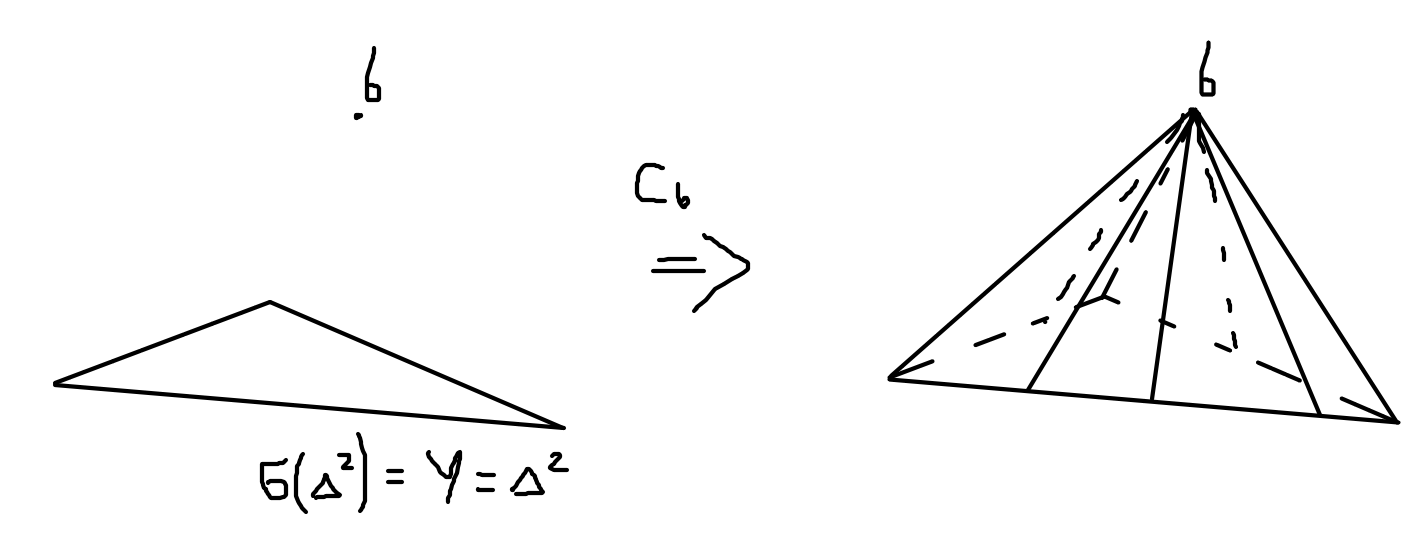
\includegraphics[scale=0.2]{cone_operator.png}
\caption*{Саме з цієї геометричної інтерпретації випливає назва оператора. Всі точки симплекса приєднуються до $b$.}
\end{figure}

\subsubsection{Гомоморфізм розбиття}
Це й буде нашим барицентричним розбиттям. Визначимо $S \colon LC_n(Y) \to LC_n(Y)$ індуктивним чином по $n$. Ми визначимо $S(\lambda) = b_\lambda(S\partial \lambda)$, де $b_\lambda \colon LC_{n-1}(Y) \to LC_n(Y)$ -- оператор конуса, а точка $b_\lambda$ -- барицентр симплекса $\lambda$. Початок індукції буде таким: $S \colon LC_{-1}(Y) \to LC_{-1}(Y)$ визначається як $S[\emptyset] = [\emptyset]$. А далі справжня база індукції: $S \colon LC_0(Y) \to LC_0(Y)$ визначимо як $S[w_0] = w_0(S\partial[w_0])$. Зауважимо, що в цьому випадку $S[w_0] = [w_0]$.\\
Доведемо, що $S$ -- ланцюгове відображення між $LC(Y)$ та на себе. Тобто покажемо, що $\partial S = S \partial$. На $LC_{-1}(Y),\ LC_0(Y)$ маємо $S = \mathbbm{1}$, тому там все автоматом. Інакше індуктивним чином маємо:\\
$\partial S (\lambda) = \partial (b_\lambda(S \partial \lambda)) = S \partial \lambda - b_\lambda \partial (S \partial \lambda) = S \partial \lambda - b_\lambda S(\partial \partial \lambda) = S \partial \lambda$.
\begin{figure}[H]
\centering
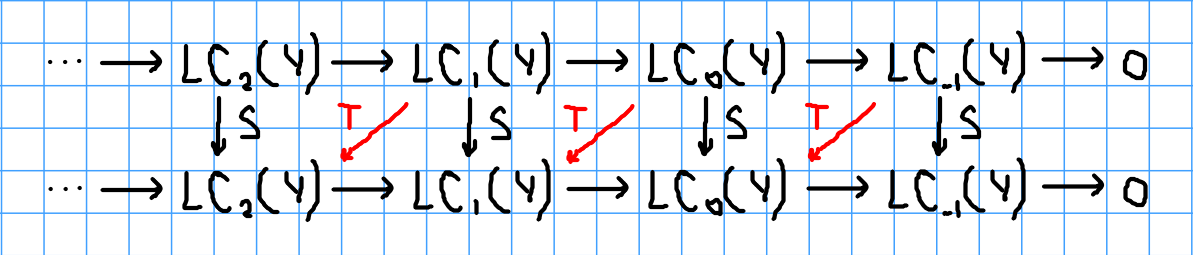
\includegraphics[scale=0.3]{chain_map_subdivision.png}
\end{figure}
Якщо $\lambda = [w_0,\dots,w_n]$ -- реальний геометричний $n$-симплекс, то тоді $S(\lambda)$ визначається як сума $n$-симплексів, які належать барицентричному розбиттю симплекса $[w_0,\dots,w_n]$ (крок 1).\\
Щоб пояснити таку індуктивну формулу, її можна порівняти з першим кроком (барицентричне розбиття симплекса). Наприклад, беремо відрізок $[w_0,w_1]$, діємо на нього $S$ -- отримуємо набір $[w_0,b], [b,w_1]$, де $b$ -- барицентр відрізка. Ці утворені розбиті відрізки віднімаються чи додаються, знак визначити можна спокійно.

\subsubsection{Гомотопія ланцюгів}
Визначимо відображення $T \colon LC_n(Y) \to LC_{+1}(Y)$. При $n = -1$ покладемо $T = 0$ та при $n \geq 0$ покладемо $T\lambda = b_\lambda(\lambda - T\partial \lambda)$. Доведемо, що $T$ -- ланцюгова гомотопія між $S$ та $\mathbbm{1}$, тобто хочемо $\partial T + T \partial = \mathbbm{1} - S$.\\
При $n = -1$ все цілком зрозуміло. При $n \geq 0$ індуктивним чином маємо\\
$\partial T\lambda = \partial b_\lambda (\lambda - T \partial \lambda) = \lambda - T \partial \lambda - b_\lambda \partial(\lambda - T \partial \lambda) = \lambda - T \partial \lambda - b_\lambda(\partial \lambda - \partial T(\partial \lambda)) = \\ = \lambda - T \partial \lambda - b_\lambda( S(\partial \lambda) + T \partial (\partial \lambda)) = \lambda - T\partial \lambda - S\lambda$.\\
На даному етапі вже можна прибрати допоміжне $LC_{-1}(Y)$. Рівність $\partial T + T \partial = \mathbbm{1} - S$ все одно виконується, бо $T = 0$ на $LC_{-1}(Y)$.\\
У геометрію поки залізати не будемо, оскільки тут важка справа.

\subsection{Барицентричне розбиття (усіх) ланцюгів}
Тепер ми повертаємось до довільного топологічного простору $X$. Ми хочемо барицентричне розбиття. Визначимо $S \colon C_n(X) \to C_n(X)$ ось таким чином: $S(\sigma) = \sigma_{\#} S([e_0,\dots,e_n])$. Трохи детальніше. Оскільки $\Delta^n$ -- частинний випадок випуклого простору, то на нього вже можна визначити $S \colon LC_n(\Delta^n) \to LC_n(\Delta^n)$, як це було вище. Маючи $\sigma \colon \Delta^n \to X$, ми породжуємо $\sigma_{\#} \colon C_n(\Delta^n) \to C_n(X)$. У нас все одно $S$ залишається ланцюговим відображенням. Дійсно\\
$\partial S \sigma = \partial \sigma_{\#} S[e_0,\dots,e_n] \overset{\partial \sigma_{\#} = \sigma_{\#} \partial}{=} \sigma_{\#} \partial S [e_0,\dots,e_n] \overset{\partial S = S \partial \text{для випуклих}}{=} \sigma_{\#} S \partial [e_0,\dots,e_n] = \\ = \sigma_{\#} \displaystyle S \left( \sum_i (-1)^i [e_0,\dots,\hat{e}_i,\dots,e_n] \right) = \sum_i (-1)^i \sigma_{\#} S [e_0,\dots,\hat{e}_i,\dots,e_n] = \sum_i (-1)^i S(\sigma|_{[e_0,\dots,\hat{e}_i,\dots,e_n]}) \\
= S\left( \sum_i (-1)^i \sigma|_{[e_0,\dots,\hat{e}_i,\dots,e_n]}\right) = S \partial \sigma$.
\bigskip \\
Визначимо схожим чином $T \colon C_n(X) \to C_{n+1}(X)$ ось так: $T\sigma = \sigma_{\#} T[e_0,\dots,e_n]$. Це все одно задаватиме гомотопію ланцюгів між $S$ та $\mathbbm{1}$. Дійсно,\\
$\partial T \sigma = \partial \sigma_{\#} T[e_0,\dots,e_n] \overset{\partial \sigma_{\#} = \sigma_{\#} \partial}{=} \sigma_{\#} \partial T [e_0,\dots,e_n] \overset{\partial T + T \partial = \mathbbm{1} - S \text{ для випуклих}}{=} \\ = \sigma_{\#} \left( [e_0,\dots,e_n] - S[e_0,\dots,e_n] - T \partial [e_0,\dots,e_n]\right) = \sigma - S \sigma - \sigma_{\#} T \partial [e_0,\dots,e_n] = \sigma - S\sigma - T(\partial \sigma)$.\\
Рівність $\sigma_{\#} T \partial [e_0,\dots,e_n] = T(\partial \sigma)$ уже рахували вище, просто замість $T$ стояла літера $S$.

\subsection{Ітеративне барицентричне розбиття}
У нас вже є гомотопія ланцюгів між $\mathbbm{1}$ та $S$ (інтуїтивно кажучи, ми провели одне розбиття). А хочеться більше, тобто зробити гомотопію ланцюгів між $\mathbbm{1}$ та $S^m$. Для цього ми задамо оператор $D_m = \displaystyle\sum_{0 \leq i < m} TS^i$. Для нього виконується $\partial D_m + D_m \partial = \mathbbm{1} - S^m$.\\
$\partial D_m + D_m \partial = \displaystyle\sum_{0 \leq i < m} \left( \partial TS^i + TS^i \partial \right) = \sum_{0 \leq i < m} \left( \partial TS^i + T\partial S^i\right) = \sum_{0 \leq i < m} (\partial T + T \partial)S^i = \sum_{0 \leq i < m} (\mathbbm{1} - S)S^i = \sum_{0 \leq i < m} (S^i - S^{i+1}) = \mathbbm{1} - S^m$.
\bigskip \\
Тепер, нарешті, ми можемо довести другу теорему. Для кожного сингулярного $\sigma \colon \Delta^n \to X$ існує таке $m$, для якого $S^m \sigma \in C_n^{\mathcal{U}}(X)$. Зараз детальне пояснення. Оскільки $\Delta^n$ -- компакт та $\sigma^{-1}(\Int U_j)$ утворюють покриття $\Delta^n$, то існує число Лебега $\delta$. Ми можемо зробити так, щоб діаметри симплексів $S^m[e_0,\dots,e_n]$ були менші за $\delta$ при достатньо великому $m$. На жаль, для кожного $\sigma$ там може бути свій $m$. Тому позначимо $m(\sigma)$ за найменше можливе число $m$, для якого $S^m \sigma \in C_n^{\mathcal{U}}(X)$.\\
Визначимо $D \colon C_n(X) \to C_{n+1}(X)$ таким чином: $D\sigma = D_{m(\sigma)} \sigma$. Для нього ми хочемо знайти відображення ланцюгів $\rho \colon C_n(X) \to C_n(X)$, де $\Im \rho = C_n^\mathcal{U}(X)$ та задовольняє $\partial D + D \partial = \mathbbm{1} - \rho$.\\
Можемо прямолінійно покласти $\rho = \mathbbm{1} - \partial D - D \partial$. Це дійсно відображення ланцюгів.\\
$\partial \rho(\sigma) = \partial \sigma - \partial^2 D\sigma - \partial D\partial \sigma = \partial \sigma - \partial D \partial \sigma$;\\
$\rho(\partial\sigma) = \partial \sigma - \partial D \partial \sigma - D \partial^2 \sigma = \partial \sigma - \partial D \partial \sigma$.
Залишилось з'ясувати, чому $\Im \rho = C_n^\mathcal{U}(X)$. Маємо:\\
$\rho(\sigma) = \sigma - \partial D \sigma - D(\partial \sigma) = \sigma - \partial D_{m(\sigma)}\sigma - D(\partial \sigma) \overset{\partial D_m + D_m \partial = \mathbbm{1} - S^m}{=} S^{m(\sigma)}\sigma + D_{m(\sigma)}(\partial \sigma) - D(\partial \sigma)$.\\
По-перше, $S^{m(\sigma)}\sigma \in C_n^{\mathcal{U}}(x)$, просто за означенням $m(\sigma)$. По-друге, розглянемо на вираз $D_{m(\sigma)} (\partial \sigma) - D(\partial \sigma)$: вони (якщо це розписати) є лінійними комбінаціями виразів $D_{m(\sigma)}(\sigma_j) - D_{m(\sigma_j)}(\sigma_j)$, де $\sigma_j = \sigma|_{[e_0,\dots,\hat{e}_j,\dots,e_n]}$ (а тому звідси $m(\sigma) \geq m(\sigma_j)$). Внаслідок чого отримуємо $D_{m(\sigma)}(\sigma_j) - D_{m(\sigma_j)}(\sigma_j) = \displaystyle\sum_{m(\sigma_j) \leq i < m(\sigma)} TS^{i}(\sigma_j)$, де кожний доданок $TS^i(\sigma_j) \in C_n^\mathcal{U}(X)$.

\subsection*{Повертаємося до першої теореми}
Точніше, повертаємось до еквівалентної версії першої теореми.
\begin{proof}
Маємо $X$ -- топологічний простір та $\mathcal{U} = \{A,B\}$ -- сім'я підпросторів, де їхні внутрішньості утворюють покриття $X$. Тоді ми знаємо, що $\partial D + D \partial = \mathbbm{1} - \imath \rho$ та $\rho \imath = \mathbbm{1}$ (внаслідок чого $\imath$ став ізоморфізмом). Всі відображення з рівностей переводять ланцюг в $A$ знову в ланцюг в $A$. Тому всі ці відображення індукують факторвідображення, вони задовольняють такі самі дві рівності. Тому факторвкладення $C_n^\mathcal{U}(X)/_{C_n(A)} \hookrightarrow C_n(X)/_{C_n(A)}$ задає ізоморфізм. Відображення ${C_n(B)}/_{C_n(A \cap B)} \to {C_n^\mathcal{U}(X)}/_{C_n(A)}$ задає ізоморфізм, бо ці групи -- вільні, де базисом будуть сингулярні симплекси $B$, які не лежать в $A$. Отже, $H_n(B, A \cap B) \cong H_n(X,A)$. 
\end{proof}
\end{document}